% questions.tex —— 2015 年·天津卷·文科 · 题目内容片段（无答案）
% 由 tools/generate_projects.py 依来源总账自 2015/2015_数学真题_天津文_试题.md 生成，勿手改（改源 MD 后重跑）


\gkpart{数学}

\begin{gktip}
\textbf{来源说明}：本题面依据固定源 PDF 全 2 页逐题核对（p1＝页 987：栏 1 标题与「一、选择题」1–5（含第 3 题框图）＋第 6 题题干末两行；栏 2 第 6 题圆图与选项、第 7–8 题＋「二、填空题」9–14（含第 10 题三视图）；栏 3「三、解答题」15、16；p2＝页 988：栏 1 第 17 题（含立体图）、第 18 题；栏 2 第 19 题；栏 3 第 20 题）。原卷为 \textbf{A3 横向（1190.55 \(\times\) 841.89 pt）三栏书刊合排}，阅读序＝左→中→右；\textbf{页脚仅印合订本书页页码 987／988}（页面底部正中），\textbf{无页眉}。标题「2015 普通高等学校招生考试（天津卷文）」在栏 1 内排印。\textbf{全卷不印分值、不印题量、不印「考生注意」栏}——三处节头逐字仅「一、选择题」「二、填空题」「三、解答题」；总分 150 为结构推断，\textbf{卷面无凭据}，本文件不作补写。

\textbf{源制作体系判定}（\texttt{pdffonts}／\texttt{pdftotext -layout}／\texttt{pdfimages -list} 实测）：源\textbf{不是扫描件，而是 LaTeX（Computer Modern 系）重排产物}——\texttt{pdfimages -list} 零命中（全页无位图，无 Type3 字体）；嵌入字体含中文 \textbf{STSong（宋体正文）／STHeiti（黑体标题与节头）}，拉丁与数学 \textbf{LMRoman 系与 CM 系（CMR10／CMMI10／CMSY10／CMEX10／MSAM10／CMR7／CMMI7 等）}，另有 \textbf{TeX-vect10}（专供向量长箭头绘制）。文本层整体可读；根号上划线、作答空线、\textbf{「$\parallel$」「$\perp$」}（第 13、17 题）、全部箭头与向量箭杆均为矢量路径。

\textbf{标点与字样约定（实测）}：① \textbf{题号与句末}源内为半角 \texttt{.}（LMRoman10 出字），按全库约定写作全角「．」；② \textbf{正文句读}源内为半角 ASCII（\texttt{, : ; ?}）与半角圆括号（\texttt{pdftotext -bbox} 与内容流双证：逗号墨迹宽 2.44 pt、出的正是 LMRoman10 的 \texttt{<002d>} 码位），本文件按全库约定归一为全角「，」「：」「；」「？」「（）」，\textbf{顿号「、」与引号「“”」为全角 CJK·照源保留}（第 15 题事件引号照源全角），内容零改动；③ \textbf{选择题选项标号}源内为\textbf{半角「(A)」照录}；④ \textbf{作答空}：填空题为统一长度横线（实测 \textbf{31.50 pt}，写作 \texttt{\gkblank{}}），选择题作答括注按全库约定写作「（　）」；⑤ \textbf{分数}源内均为显示风格（真分式：第 5 题分数线 10.5–26.3 pt、第 13 题两系数分子分母全字号），排印一律按显示风格（如 \(\dfrac{a}{b}\)）；⑥ \textbf{不等号}按 MSAM10 实测字形排 \(\leqslant\)（字形名 \texttt{lessorequalslant}，U+2A7D；第 2、3、8、20 题；同子集含 \texttt{greaterorequalslant} 备用）；⑦ \textbf{向量}：本卷源\textbf{无 CMMIB10}——向量字母为 \textbf{CMMI10 常规数学斜体}、箭杆为 \textbf{TeX-vect10 长箭头}，一律录作 \(\overrightarrow{BE}\) 类（\textbf{不加粗斜体向量记号}）；⑧ \textbf{常数与函数名}：\(\log\)／\(\sin\)／\(\cos\)／\(\ln\) 源为\textbf{正体}（LMRoman10／CMR10），照录正体；实数集与正整数集源为\textbf{粗正体}（LMRoman10-Bold），录作 \(\mathbf{R}\)／\(\mathbf{N}^*\)；补集号 \(\complement\) 出自 MSAM10（字形名 \texttt{complement}，U+2201）；⑨ \textbf{第 15 题}的 ①② 为圈号字形；⑩ \textbf{第 18 题}的 \(A_1,\dots,A_6\) 下标与 \(\mathbf{N}^*\) 上标照源；⑪ \textbf{词间空格}照页面词界补。

\textbf{存疑与登记}（源内异常一律照录；完整清单见工作档 \texttt{figure-inventory.md} 存疑表 S-1…S-10 与转录稿存疑表）：① \textbf{固定源不附参考答案}（等级 D）——本题面无答案区，解析全部由本库独立推导；② \textbf{第 3 题源内矛盾}：题干问「则输出 \(i\) 的值为」，而程序框图的输出框内印「\textbf{输出 \(S\)}」（600 dpi 渲染与文本层双证一致；若严格按框内输出则为 \(S=0\)，不在选项 2/3/4/5 之列）——\textbf{照源复刻、不作改动}，判读与答案处置见《答案要点》与解析正文登记（纯题面版不印答案值）；③ \textbf{第 6 题图}：标签 \(C\) 落在圆轮廓外（紧邻下方），题干称「弦 \(CD\)，\(CE\)」——\(C\) 系两弦公共端点、应在圆上，标签因避让线段外移，\textbf{照源复刻}（图清单实测 \(C/D/E\) 三点落圆偏差 \(\leqslant0.06\) pt）；④ \textbf{第 13、17 题的「$\parallel$」}在文本层被整体吞掉（pdftotext 输出「AB DC」「BB1 AA1」「EF 平面 A1B1BA」），渲染图实测符号均在——\textbf{凡平行记号一律以渲染图为准}；⑤ \textbf{第 20 题 (3) 末项指数}在文本层被打散错排，渲染图实测为 \textbf{\(4^{\frac{1}{3}}\)}（指数位「1 在上、3 在下」的竖排小分式，分数杆线宽 0.3387 w 为全卷唯一；\textbf{非立方根号形}）；⑥ 全卷标点为半角拉丁字形，已按全库约定归一全角（源形在转录稿登记）；⑦ 全卷无分值印制，不录不补。
\end{gktip}

\gkpart{试题}

\gkpart{一、选择题}

\begin{question}
\gkti{1}已知全集 \(U=\{1,2,3,4,5,6\}\)，集合 \(A=\{2,3,5\}\)，集合 \(B=\{1,3,4,6\}\)，则集合 \(A\cap\complement_U B=\)（　）

(A) \(\{3\}\)　(B) \(\{2,5\}\)　(C) \(\{1,4,6\}\)　(D) \(\{2,3,5\}\)

\end{question}
\begin{question}
\gkti{2}设变量 \(x\)，\(y\) 满足约束条件 \(\begin{cases}x-2\leqslant0,\\x-2y\leqslant0,\\x+2y-8\leqslant0,\end{cases}\) 则目标函数 \(z=3x+y\) 的最大值为（　）

(A) 7　(B) 8　(C) 9　(D) 14

\Needspace{0.4\textheight}
\end{question}
\begin{question}
\gkti{3}阅读程序框图，运行相应的程序，则输出 \(i\) 的值为（　）
\nopagebreak[4]
\begin{center}% f2015tjw_q03_flowchart.tex —— 2015 天津文科卷 Q3 程序框图（源 p1 栏 1）
%
% 源：.work/phase3-b10/source/2015天津文.pdf（p1 印 987）；实测清单 figure-inventory.md §F01
% 坐标换算：x_pic = x_pt − 175.534 ；y_pic = 542.040 − y_pt
%   （源页 pt、原点左上、y 向下；y 取反并平移，使图内画布 y 向上；
%     画布范围 x' 0.000–95.833、y' 0.147–204.730，单位 pt）
% 线宽：0.398 pt（源 `0.398 w` 实测；全图实线，p1 无虚线）
% 箭头：TikZ 标准 `>=stealth`（既定重绘约定）。
%   源箭尖为 8 点填充多边形（实测 2.88–3.36 宽 × 3.6–4.0 长），其内容流提取坐标与墨迹不符
%   （清单 §S-1：沿线采样仅 15.42% 落墨）。本文件**不采用提取值**，箭尖落点一律由本次
%   600 dpi 墨迹独立实测（口径：沿轴扫描，取墨迹最远端；见 .work/phase3-b10/probe/arrowtips 系）：
%     C1 起 (216.223, 354.347) 尖 368.16 ｜ C2 起 (216.223, 385.120) 尖 398.88
%     C3 起 (216.223, 414.491) 尖 428.28 ｜ C4 起 (216.223, 444.113) 尖 457.92
%     C5 起 (216.223, 479.071) 尖 492.84 ｜ C6 起 (216.223, 510.504) 尖 524.28
%     否支折线 3 段，尖 x = 216.96（源提取值 223.396 系偏移值，已弃用）
%   （六枚主链箭尖与目标框边的墨迹间隙均 0.36 pt；C4 与菱形上顶点同）
% 存疑照源复刻：否支出口 N1 起点 x=257.194 与菱形右顶点 256.913 差 0.281 pt；
%   否支落点在 B2/B3 之间的竖段上（y=392.206）；标签「是」在菱形下方、「否」在菱形右侧 —— 均按源。
\begin{tikzpicture}[x=1pt, y=1pt, line width=0.398pt, >=stealth, every node/.style={font=\fontsize{10.5pt}{12.6pt}\selectfont,inner sep=0pt}]

  % ---- 七个框 ----
  \draw[rounded corners=3.985pt] (26.690,204.730) rectangle (54.689,187.892);   % B1 开始
  \draw (6.776,173.320) rectangle (74.603,157.119);                             % B2 S=10,i=0
  \draw (17.530,142.547) rectangle (63.848,127.748);                            % B3 i=i+1
  \draw (14.920,113.176) rectangle (66.458,98.127);                             % B4 S=S-i
  \draw (81.379,73.362) -- (40.689,83.473) -- (0.000,73.362)
        -- (40.689,63.251) -- cycle;                                            % B5 菱形 S<=1?
  \draw (15.281,31.736) -- (21.417,48.595) -- (66.092,48.595)
        -- (59.957,31.736) -- cycle;                                            % B6 输出 S（平行四边形）
  \draw[rounded corners=3.985pt] (26.690,17.163) rectangle (54.689,0.147);      % B7 结束

  % ---- 主链 6 段（箭尖落点见文件头实测值） ----
  \draw[->] (40.689,187.693) -- (40.689,173.880);   % 354.347 -> 尖 368.16
  \draw[->] (40.689,156.920) -- (40.689,143.160);   % 385.120 -> 尖 398.88
  \draw[->] (40.689,127.549) -- (40.689,113.760);   % 414.491 -> 尖 428.28
  \draw[->] (40.689, 97.927) -- (40.689, 84.120);   % 444.113 -> 尖 457.92
  \draw[->] (40.689, 62.969) -- (40.689, 49.200);   % 479.071 -> 尖 492.84
  \draw[->] (40.689, 31.536) -- (40.689, 17.760);   % 510.504 -> 尖 524.28

  % ---- 「否」支：3 折段回环，落于 B2 与 B3 之间竖段 ----
  \draw[->] (81.660,73.362) -- (95.833,73.362) -- (95.833,149.834) -- (41.426,149.834);

  % ---- 标签（源 pdftotext -bbox 字形盒左上角；inner sep=0） ----
  \node[anchor=north west,inner sep=0] at (30.186,202.140) {开始};
  \node[anchor=north west,inner sep=0] at (10.276,169.930) {$S=10,\,i=0$};
  \node[anchor=north west,inner sep=0] at (21.026,139.410) {$i=i+1$};
  \node[anchor=north west,inner sep=0] at (18.416,109.790) {$S=S-i$};
  \node[anchor=north west,inner sep=0] at (25.066, 80.350) {$S\leqslant 1\,?$};
  \node[anchor=north west,inner sep=0] at (44.386, 61.820) {是};
  \node[anchor=north west,inner sep=0] at (76.406, 70.890) {否};
  \node[anchor=north west,inner sep=0] at (24.916, 46.030) {输出 $S$};
  \node[anchor=north west,inner sep=0] at (30.186, 14.510) {结束};

\end{tikzpicture}
\end{center}
\nopagebreak[4]
(A) 2　(B) 3　(C) 4　(D) 5

\end{question}
\begin{question}
\gkti{4}设 \(x\in\mathbf{R}\)，则“\(1<x<2\)”是“\(|x-2|<1\)”的（　）

(A) 充分而不必要条件　(B) 必要而不充分条件

(C) 充要条件　(D) 既不充分也不必要条件

\end{question}
\begin{question}
\gkti{5}已知双曲线 \(\dfrac{x^2}{a^2}-\dfrac{y^2}{b^2}=1\)（\(a>0\)，\(b>0\)）的一焦点为 \(F(2,0)\)，且双曲线的渐近线与圆 \((x-2)^2+y^2=3\) 相切，则双曲线的方程为（　）

(A) \(\dfrac{x^2}{9}-\dfrac{y^2}{13}=1\)　(B) \(\dfrac{x^2}{13}-\dfrac{y^2}{9}=1\)

(C) \(\dfrac{x^2}{3}-y^2=1\)　(D) \(x^2-\dfrac{y^2}{3}=1\)

\Needspace{0.4\textheight}
\end{question}
\begin{question}
\gkti{6}如图，在圆 \(O\) 中，\(M\)，\(N\) 是弦 \(AB\) 的三等分点，弦 \(CD\)，\(CE\) 分别经过点 \(M\)，\(N\)，若 \(CM=2\)，\(MD=4\)，\(CN=3\)，则线段 \(NE\) 的长为（　）
\nopagebreak[4]
\begin{center}% f2015tjw_q06_circle.tex —— 2015 天津文科卷 Q6 圆与割线图（源 p1 栏 2）
%
% 源：.work/phase3-b10/source/2015天津文.pdf（p1 印 987）；实测清单 figure-inventory.md §F02
% 坐标换算：x_pic = x_pt − 535.0 ；y_pic = 200.0 − y_pt
%   （源页 pt、原点左上、y 向下；画布 x' 0.05–119.8、y' 12.5–139.9，单位 pt）
% 线宽：0.398 pt（源 `0.398 w` 实测）；无箭头、无虚线（p1 全页 `[] 0 d`）。
% 几何：圆心 O=(60.122, 76.348)，R=53.892；弦 AB 水平 y'=59.339；
%   三等分点 M=(43.056, 59.339)、N=(77.188, 59.339)（由 A 端按 1/3、2/3 内插）；
%   两割线共点 C=(42.262, 25.490)，另端 D=(49.747, 129.247)、E=(111.320, 93.357)。
%   三点落圆校验（清单实测）：C 半径 53.904、D 53.907、E 53.949（R=53.892，偏差 ≤0.06 pt）。
% 存疑照源复刻：§S-4 圆心「•」在源中是**文字字形**而非矢量圆点 —— 故本文件同样以文字绘制，
%   按源字形盒左上角 (58.55, 80.93) 定位，不用 \fill circle。
%   另：C 标签落在圆轮廓外、A/B 标签在弦端点外侧，均按源字形盒原样定位。
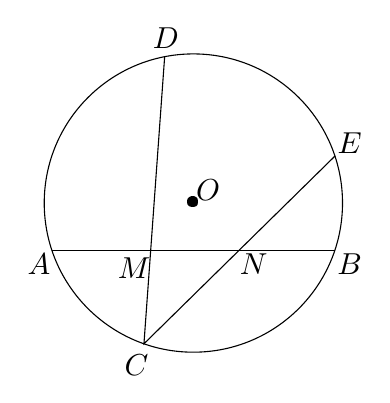
\begin{tikzpicture}[x=1pt, y=1pt, line width=0.398pt, every node/.style={font=\fontsize{10.5pt}{12.6pt}\selectfont,inner sep=0pt}]

  % ---- 圆 ----
  \draw (60.122,76.348) circle [radius=53.892];

  % ---- 弦 AB（A、B 恰在圆上） ----
  \draw (8.924,59.339) -- (111.320,59.339);

  % ---- 两条割线 CD、CE（共用 C，一条折线） ----
  \draw (49.747,129.247) -- (42.262,25.490) -- (111.320,93.357);

  % ---- 圆心墨点（源为文字字形而非矢量圆点，§S-4；故此处同样以文字绘制） ----
  % 源墨迹实测：圆盘 2.28 pt 见方、面积 4.68 pt^2、质心 (595.030, 123.445)；字形盒左上 (593.55,119.07)
  % 本稿按源「墨迹质心」定位（anchor=center），与源字形盒定位的差 0.2 pt 量级；
  % 探针 600dpi 复测：本稿墨点面积 4.46 pt^2、质心距源质心 0.94 pt（同量级，登记备终检微调）
  \node[anchor=center,inner sep=0] at (60.030,76.555) {\textbullet};

  % ---- 标签（源 pdftotext -bbox 字形盒左上角；inner sep=0） ----
  \node[anchor=north west,inner sep=0] at (45.25,139.92) {$D$};
  \node[anchor=north west,inner sep=0] at (112.07,101.99) {$E$};
  \node[anchor=north west,inner sep=0] at (60.90, 84.98) {$O$};
  \node[anchor=north west,inner sep=0] at ( 0.05, 58.11) {$A$};
  \node[anchor=north west,inner sep=0] at (32.64, 56.70) {$M$};
  \node[anchor=north west,inner sep=0] at (76.76, 58.11) {$N$};
  \node[anchor=north west,inner sep=0] at (112.00,58.11) {$B$};
  \node[anchor=north west,inner sep=0] at (35.09, 21.83) {$C$};

\end{tikzpicture}
\end{center}
\nopagebreak[4]
(A) \(\dfrac{8}{3}\)　(B) 3　(C) \(\dfrac{10}{3}\)　(D) \(\dfrac{5}{2}\)

\end{question}
\begin{question}
\gkti{7}已知定义在 \(\mathbf{R}\) 上的函数 \(f(x)=2^{|x-m|}-1\)（\(m\) 为实数）为偶函数，记 \(a=f(\log_{0.5}3)\)，\(b=f(\log_2 5)\)，\(c=f(2m)\)，则 \(a\)，\(b\)，\(c\) 的大小关系为（　）

(A) \(a<b<c\)　(B) \(c<a<b\)　(C) \(a<c<b\)　(D) \(c<b<a\)

\end{question}
\begin{question}
\gkti{8}已知函数 $f(x)=\begin{cases}2-|x|,&x\leqslant2,\\(x-2)^2,&x>2,\end{cases}$ 函数 \(g(x)=3-f(2-x)\)，则函数 \(y=f(x)-g(x)\) 的零点个数为（　）

(A) 2　(B) 3　(C) 4　(D) 5

\end{question}
\gkpart{二、填空题}

\begin{question}
\gkti{9}\(\mathrm{i}\) 是虚数单位，计算 \(\dfrac{1-2\mathrm{i}}{2+\mathrm{i}}\) 的结果为\gkblank{}．

\Needspace{0.4\textheight}
\end{question}
\begin{question}
\gkti{10}一个几何体的三视图如图所示（单位：m），则该几何体的体积为\gkblank{}m³．
\nopagebreak[4]
\begin{center}% f2015tjw_q10_views.tex —— 2015 天津文科卷 Q10 三视图（源 p1 栏 2）
%
% 源：.work/phase3-b10/source/2015天津文.pdf（p1 印 987）；实测清单 figure-inventory.md §F03
% 坐标换算：x_pic = x_pt − 490.0 ；y_pic = 605.0 − y_pt
%   （源页 pt、原点左上、y 向下；画布 x' 3.36–197.7、y' 6.74–195.59，单位 pt）
% 线宽：0.398 pt（源 `0.398 w` 实测）；全图实线（p1 无虚线）。
% 结构：正视图六边形 + 侧视图圆（含半径引导线）+ 俯视图六边形（= 正视图整体下移 113.388 pt）
%   ＋三组刻度＋左右竖尺寸线与横向尺寸链。
% 箭头：TikZ 标准 `>=stealth`（既定重绘约定）。源箭尖为 8 点填充多边形（实测 2.88–3.36 宽 ×
%   3.6–4.0 长），其提取坐标与墨迹不符（清单 §S-1：沿线采样仅 19.22% 落墨）；
%   本文件**不采用提取值**，24 枚中每一枚均由本次 600 dpi 墨迹独立实测（沿轴扫描取墨迹最远端）：
%     正/俯视图左右竖尺寸线 16 枚：尖分别落于对应刻度 y（实测值见下 16 行注释；与刻度的墨迹
%       间隙 0.00–0.52 pt，其中 6 枚与刻度墨迹直接相接，系尖点抗锯齿衰减，端点取刻度的几何 y）
%     横向尺寸链 6 枚（y_pt = 471.776）：尖分别为 501.860(←)、530.207(→)、530.207(←)、
%       586.900(→)、586.900(←)、615.247(→)——即**每枚尖都落在同侧刻度上**
%     侧视图半径 1 枚：尖实测 (691.00, 418.56)（距圆心 27.05，R=28.347）
%   注：600 dpi 墨迹全图（x 490–700, y 405–600）共检出**23 枚**实心箭尖（4+4 竖[正视]、4+4 竖[俯视]、
%   横向链 6、半径 1）。内容流提取计数为 24，多出的 1 枚为横向尺寸链上的「另 1 个」；
%   墨迹中不存在该枚（横向链的 6 段各只配 1 枚，两两指向同一刻度），登记为提取侧幻影。
% 存疑照源复刻：§S-7 半径箭尖距圆心 27.05 < R=28.347（箭头内缩）；§S-8 横向链 6 段长度与
%   「1|2|1」标注不成正比；§S-9 正/俯视图间距不对应「长对正、高平齐」——均按源不修正。
\begin{tikzpicture}[x=1pt, y=1pt, line width=0.398pt, >=stealth, every node/.style={font=\fontsize{10.5pt}{12.6pt}\selectfont,inner sep=0pt}]

  % ---- 正视图（六边形 + 两条内竖线） ----
  \draw (11.860,167.240) -- (40.207,138.893) -- (96.900,138.893) -- (125.247,167.240)
        -- (96.900,195.587) -- (40.207,195.587) -- cycle;
  \draw (40.207,138.893) -- (40.207,195.587);
  \draw (96.900,138.893) -- (96.900,195.587);

  % ---- 侧视图（圆 + 半径引导线，箭尖＝墨迹实测 (691.00,418.56)） ----
  \draw (181.941,167.240) circle [radius=28.347];
  \draw[->] (181.941,167.240) -- (201.000,186.440);

  % ---- 俯视图（同上六边形整体下移 113.388 pt） ----
  \draw (11.860,53.852) -- (40.207,25.505) -- (96.900,25.505) -- (125.247,53.852)
        -- (96.900,82.199) -- (40.207,82.199) -- cycle;
  \draw (40.207,25.505) -- (40.207,82.199);
  \draw (96.900,25.505) -- (96.900,82.199);

  % ---- 刻度：正视图左/右各 3、顶边 4；俯视图左/右各 3 ----
  \draw (3.356,138.893) -- (9.025,138.893);    \draw (128.082,138.893) -- (133.751,138.893);
  \draw (3.356,167.240) -- (9.025,167.240);    \draw (128.082,167.240) -- (133.751,167.240);
  \draw (3.356,195.587) -- (9.025,195.587);    \draw (128.082,195.587) -- (133.751,195.587);
  \draw (11.860,130.389) -- (11.860,136.058);  \draw (40.207,130.389) -- (40.207,136.058);
  \draw (96.900,130.389) -- (96.900,136.058);  \draw (125.247,130.389) -- (125.247,136.058);
  \draw (3.356,25.506) -- (9.025,25.506);      \draw (128.082,25.506) -- (133.751,25.506);
  \draw (3.356,53.852) -- (9.025,53.852);      \draw (128.082,53.852) -- (133.751,53.852);
  \draw (3.356,82.199) -- (9.025,82.199);      \draw (128.082,82.199) -- (133.751,82.199);

  % ---- 正视图左右竖尺寸线（各 4 段，箭尖落于刻度；括号内为 600dpi 墨迹实测尖 y_pt） ----
  \draw[->] (130.917,147.397) -- (130.917,138.893);   % 457.603 -> 尖 465.96, 刻度 466.107
  \draw[->] (130.917,158.736) -- (130.917,167.240);   % 446.264 -> 尖 438.00, 刻度 437.760
  \draw[->] (130.917,175.744) -- (130.917,167.240);   % 429.256 -> 尖 437.28, 刻度 437.760
  \draw[->] (130.917,187.083) -- (130.917,195.587);   % 417.917 -> 尖 409.44, 刻度 409.413
  \draw[->] (  6.191,147.397) -- (  6.191,138.893);   % 同上（左，实测 465.96）
  \draw[->] (  6.191,158.736) -- (  6.191,167.240);   % 同上（左，实测 438.00）
  \draw[->] (  6.191,175.744) -- (  6.191,167.240);   % 同上（左，实测 437.28）
  \draw[->] (  6.191,187.083) -- (  6.191,195.587);   % 同上（左，实测 409.44）

  % ---- 俯视图左右竖尺寸线（各 4 段） ----
  \draw[->] (130.917,34.010) -- (130.917,25.506);     % 570.990 -> 尖 579.00, 刻度 579.494
  \draw[->] (130.917,45.348) -- (130.917,53.852);     % 559.652 -> 尖 551.40, 刻度 551.148
  \draw[->] (130.917,62.357) -- (130.917,53.852);     % 542.643 -> 尖 550.92, 刻度 551.148
  \draw[->] (130.917,73.695) -- (130.917,82.199);     % 531.305 -> 尖 523.32, 刻度 522.801
  \draw[->] (  6.191,34.010) -- (  6.191,25.506);     % 同上（左，实测 579.00）
  \draw[->] (  6.191,45.348) -- (  6.191,53.852);     % 同上（左，实测 551.40）
  \draw[->] (  6.191,62.357) -- (  6.191,53.852);     % 同上（左，实测 550.92）
  \draw[->] (  6.191,73.695) -- (  6.191,82.199);     % 同上（左，实测 523.32）

  % ---- 横向尺寸链（6 段，箭尖均落在刻度上） ----
  \draw[->] (20.364,133.224) -- (11.860,133.224);     % 尖 501.860(←)
  \draw[->] (31.703,133.224) -- (40.207,133.224);     % 尖 530.207(→)
  \draw[->] (62.884,133.224) -- (40.207,133.224);     % 尖 530.207(←)
  \draw[->] (74.223,133.224) -- (96.900,133.224);     % 尖 586.900(→)
  \draw[->] (105.404,133.224) -- (96.900,133.224);    % 尖 586.900(←)
  \draw[->] (116.743,133.224) -- (125.247,133.224);   % 尖 615.247(→)

  % ---- 标签（视图名：源 pdftotext -bbox 字形盒左上角；尺寸数字：源字形盒左上角，
  %      竖线数字与半径数字的 x 由 600dpi 墨迹反推（清单只给 y 档）——inner sep=0） ----
  \node[anchor=north west,inner sep=0] at ( 52.80,122.06) {正视图};
  \node[anchor=north west,inner sep=0] at (166.19,122.07) {侧视图};
  \node[anchor=north west,inner sep=0] at ( 52.80, 17.24) {俯视图};
  \node[anchor=north west,inner sep=0] at ( 23.41,137.13) {$1$};
  \node[anchor=north west,inner sep=0] at ( 65.93,137.13) {$2$};
  \node[anchor=north west,inner sep=0] at (108.45,137.13) {$1$};
  \node[anchor=north west,inner sep=0] at (193.41,173.98) {$1$};
  \node[anchor=north west,inner sep=0] at (  3.55,185.32) {$1$};
  \node[anchor=north west,inner sep=0] at (  3.55,156.97) {$1$};
  \node[anchor=north west,inner sep=0] at (  3.55, 71.93) {$1$};
  \node[anchor=north west,inner sep=0] at (  3.55, 43.58) {$1$};
  \node[anchor=north west,inner sep=0] at (128.31,185.32) {$1$};
  \node[anchor=north west,inner sep=0] at (128.31,156.97) {$1$};
  \node[anchor=north west,inner sep=0] at (128.31, 71.93) {$1$};
  \node[anchor=north west,inner sep=0] at (128.31, 43.58) {$1$};

\end{tikzpicture}
\end{center}
\nopagebreak[4]
\end{question}
\begin{question}
\gkti{11}已知函数 \(f(x)=ax\ln x\)，\(x\in(0,+\infty)\)，其中 \(a\) 为实数，\(f'(x)\) 为 \(f(x)\) 的导函数．若 \(f'(1)=3\)，则 \(a\) 的值为\gkblank{}．

\end{question}
\begin{question}
\gkti{12}已知 \(a>0\)，\(b>0\)，\(ab=8\)，则当 \(a\) 的值为\gkblank{}时，\(\log_2 a\cdot\log_2(2b)\) 取得最大值．

\end{question}
\begin{question}
\gkti{13}在等腰梯形 \(ABCD\) 中，已知 \(AB\parallel DC\)，\(AB=2\)，\(BC=1\)，\(\angle ABC=60^{\circ}\)．点 \(E\) 和 \(F\) 分别在线段 \(BC\) 和 \(DC\) 上，且 \(\overrightarrow{BE}=\dfrac{2}{3}\overrightarrow{BC}\)，\(\overrightarrow{DF}=\dfrac{1}{6}\overrightarrow{DC}\)，则 \(\overrightarrow{AE}\cdot\overrightarrow{AF}\) 的值为\gkblank{}．

\end{question}
\begin{question}
\gkti{14}已知函数 \(f(x)=\sin\omega x+\cos\omega x\)（\(\omega>0\)），\(x\in\mathbf{R}\)，若函数 \(f(x)\) 在区间 \((-\omega,\omega)\) 内单调递增，且函数 \(y=f(x)\) 的图象关于直线 \(x=\omega\) 对称，则 \(\omega\) 的值为\gkblank{}．

\end{question}
\gkpart{三、解答题}

\begin{question}
\gkti{15}设甲、乙、丙三个乒乓球协会的运动员人数分别为 27，9，18．现采用分层抽样的方法从这三个协会中抽取 6 名运动员组队参加比赛．

（1） 求应从这三个协会中分别抽取的运动员的人数；

（2） 将抽取的 6 名运动员进行编号，编号分别为 \(A_1\)，\(A_2\)，\(A_3\)，\(A_4\)，\(A_5\)，\(A_6\)．现从这 6 名运动员中随机抽取 2 人参加双打比赛．

① 用所给编号列出所有可能的结果；

② 设 \(A\) 为事件：“编号为 \(A_5\) 和 \(A_6\) 的两名运动员中至少有 1 人被抽到”，求事件 \(A\) 发生的概率．

\end{question}
\begin{question}
\gkti{16}在 \(\triangle ABC\) 中，内角 \(A\)，\(B\)，\(C\) 所对的边分别为 \(a\)，\(b\)，\(c\)．已知 \(\triangle ABC\) 的面积为 \(3\sqrt{15}\)，\(b-c=2\)，\(\cos A=-\dfrac{1}{4}\)．

（1） 求 \(a\) 和 \(\sin C\) 的值；

（2） 求 \(\cos\left(2A+\dfrac{\pi}{6}\right)\) 的值．

\Needspace{0.4\textheight}
\end{question}
\begin{question}
\gkti{17}如图，已知 \(AA_1\perp\) 平面 \(ABC\)，\(BB_1\parallel AA_1\)，\(AB=AC=3\)，\(BC=2\sqrt{5}\)，\(AA_1=\sqrt{7}\)，\(BB_1=2\sqrt{7}\)，点 \(E\) 和 \(F\) 分别为 \(BC\) 和 \(A_1C\) 的中点．
\nopagebreak[4]
\begin{center}% f2015tjw_q17_solid.tex —— 2015 天津文科卷 Q17 立体图（源 p2 栏 1）
%
% 源：.work/phase3-b10/source/2015天津文.pdf（p2 印 988）；实测清单 figure-inventory.md §F04
% 坐标换算：x_pic = x_pt − 285.0 ；y_pic = 370.0 − y_pt
%   （源页 pt、原点左上、y 向下；画布 x' 2.7–120.2、y' 6.0–218.2，单位 pt）
% 线宽：0.3985 pt（源 `0.3985 w` 实测）；虚线用源 dash 实测节距 `[ 2.98883 2.98883 ] 0 d`
%   → dash pattern = on 2.98883pt off 2.98883pt（全卷仅本图 4 条棱为虚线）。
% 顶点（源 pt → 图内）：
%   B(299.659,320.463)→(14.659,49.537)  A(389.780,320.463)→(104.780,49.537)
%   C(367.328,351.335)→(82.328,18.665)  A₁(389.780,240.632)→(104.780,129.368)
%   B₁(299.659,160.802)→(14.659,209.198) E(333.493,335.899)→(48.493,34.101)
%   F(378.242,295.984)→(93.242,74.016)
% 实虚分工照源（不做修正）：7 实（BC、CA、B₁B、AA₁、CA₁、CB₁、A₁B₁）＋
%   4 虚（BA 底面棱、EA₁、EF、AE）＝ 11 条棱（源 22 条路径 = 11 棱 + 11 条退化 m 占位）。
% 存疑照源复刻：§S-6 F 点实测 (378.242,295.984) 与 A₁C 理论中点 (378.554,295.984) 差 x 0.312 pt；
%   E 点为 BC 中点（与题干一致，差 0.001 pt）——均按实测坐标给出。
% 全图无箭头（源 p2 图形线素无 f 填充箭尖）。
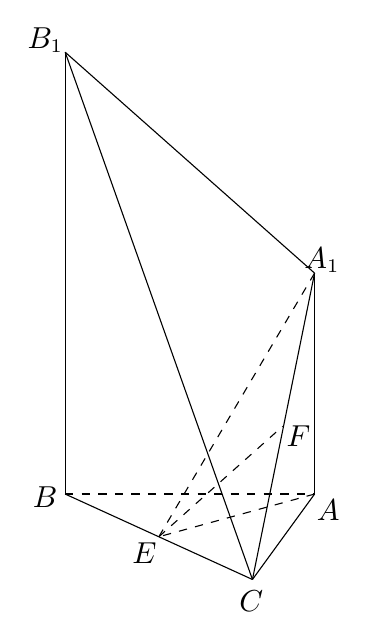
\begin{tikzpicture}[x=1pt, y=1pt, line width=0.3985pt, every node/.style={font=\fontsize{10.5pt}{12.6pt}\selectfont,inner sep=0pt}]

  % ---- 实线棱 7 条 ----
  \draw (14.659, 49.537) -- (82.328, 18.665);   % E1  B -> C
  \draw (82.328, 18.665) -- (104.780,49.537);   % E2  C -> A
  \draw (14.659,209.198) -- (14.659, 49.537);   % E3  B1 -> B
  \draw (104.780,49.537) -- (104.780,129.368);  % E4  A -> A1
  \draw (82.328, 18.665) -- (104.780,129.368);  % E5  C -> A1
  \draw (82.328, 18.665) -- (14.659,209.198);   % E6  C -> B1
  \draw (104.780,129.368) -- (14.659,209.198);  % E7  A1 -> B1

  % ---- 虚线棱 4 条（dash 2.98883 on/off，源实测） ----
  \draw[dash pattern=on 2.98883pt off 2.98883pt] (14.659,49.537) -- (104.780,49.537);   % E8  B -> A（底面）
  \draw[dash pattern=on 2.98883pt off 2.98883pt] (48.493,34.101) -- (104.780,129.368);  % E9  E -> A1
  \draw[dash pattern=on 2.98883pt off 2.98883pt] (48.493,34.101) -- (93.242, 74.016);   % E10 E -> F
  \draw[dash pattern=on 2.98883pt off 2.98883pt] (104.780,49.537) -- (48.493,34.101);   % E11 A -> E

  % ---- 标签（源标签 bbox 中心 → 最近顶点判定归属；anchor=center、inner sep=0） ----
  \node[anchor=center,inner sep=0] at (  7.42,48.57) {$B$};
  \node[anchor=center,inner sep=0] at (109.71,43.64) {$A$};
  \node[anchor=center,inner sep=0] at ( 81.95,10.73) {$C$};
  \node[anchor=center,inner sep=0] at (107.48,134.12) {$A_1$};
  \node[anchor=center,inner sep=0] at (  7.50,213.50) {$B_1$};
  \node[anchor=center,inner sep=0] at ( 43.26,28.21) {$E$};
  \node[anchor=center,inner sep=0] at ( 98.96,70.38) {$F$};

\end{tikzpicture}
\end{center}
\nopagebreak[4]
（1） 求证：\(EF\parallel\) 平面 \(A_1B_1BA\)；

（2） 求证：平面 \(AEA_1\perp\) 平面 \(BCB_1\)；

（3） 求直线 \(A_1B_1\) 与平面 \(BCB_1\) 所成角的大小．

\end{question}
\begin{question}
\gkti{18}已知数列 \(\{a_n\}\) 是各项均为正数的等比数列，\(\{b_n\}\) 是等差数列，且 \(a_1=b_1=1\)，\(b_2+b_3=2a_3\)，\(a_5-3b_2=7\)．

（1） 求 \(\{a_n\}\) 和 \(\{b_n\}\) 的通项公式；

（2） 设 \(c_n=a_nb_n\)，\(n\in\mathbf{N}^*\)，求数列 \(\{c_n\}\) 的前 \(n\) 项和．

\end{question}
\begin{question}
\gkti{19}已知椭圆 \(\dfrac{x^2}{a^2}+\dfrac{y^2}{b^2}=1\)（\(a>b>0\)）的上顶点为 \(B\)，左焦点为 \(F\)，离心率为 \(\dfrac{\sqrt{5}}{5}\)．

（1） 求直线 \(BF\) 的斜率；

（2） 设直线 \(BF\) 与椭圆交于点 \(P\)（\(P\) 异于点 \(B\)），过点 \(B\) 且垂直于 \(BP\) 的直线与椭圆交于点 \(Q\)（\(Q\) 异于点 \(B\)），直线 \(PQ\) 与 \(y\) 轴交于点 \(M\)，\(|PM|=\lambda|MQ|\)．

① 求 \(\lambda\) 的值；

② 若 \(|PM|\sin\angle BQP=\dfrac{7\sqrt{5}}{9}\)，求椭圆的方程．

\end{question}
\begin{question}
\gkti{20}已知函数 \(f(x)=4x-x^4\)，\(x\in\mathbf{R}\)．

（1） 求 \(f(x)\) 的单调区间；

（2） 设曲线 \(y=f(x)\) 与 \(x\) 轴正半轴的交点为 \(P\)，曲线在点 \(P\) 处的切线方程为 \(y=g(x)\)，求证：对于任意的实数 \(x\)，都有 \(f(x)\leqslant g(x)\)；

（3） 若方程 \(f(x)=a\)（\(a\) 为实数）有两个正实数根 \(x_1\)，\(x_2\)，且 \(x_1<x_2\)，求证：\(x_2-x_1\leqslant-\dfrac{a}{3}+4^{\frac{1}{3}}\)．

\end{question}